\documentclass[a4paper,12pt]{jarticle}

% レイアウト
\setlength{\hoffset}{0cm}
\setlength{\oddsidemargin}{-3mm}
\setlength{\evensidemargin}{-3cm}
\setlength{\marginparsep}{0cm}
\setlength{\marginparwidth}{0cm}
\setlength{\textheight}{24.7cm}
\setlength{\textwidth}{17cm}
\setlength{\topmargin}{-45pt}


\renewcommand{\baselinestretch}{1.6}
\renewcommand{\floatpagefraction}{1}
\renewcommand{\topfraction}{1}
\renewcommand{\bottomfraction}{1}
\renewcommand{\textfraction}{0}
\renewcommand\thefootnote{\arabic{footnote})}

% パッケージ
\usepackage[dvipdfmx]{graphicx}
\usepackage{amsmath,amssymb,epsfig}
\usepackage{eucal}
\usepackage{bm}
\usepackage{ascmac}
\usepackage{pifont}
\usepackage{multirow}
\usepackage{enumerate}
\usepackage{cases}
\usepackage{type1cm}
\usepackage{cancel}
\usepackage{url}
\usepackage{cite}
%\usepackage{color}
\usepackage[dvipdfmx]{color}
\usepackage{caption}
\usepackage[caption=false]{subfig}
\captionsetup[figure]{labelsep=space}
\usepackage{here}

% 擬似コード作成用
\usepackage[ruled,vlined]{algorithm2e}
\usepackage{setspace}
\DeclareRelationFont{JY1}{mc}{it}{}{OT1}{cmr}{it}{}
\DeclareRelationFont{JT1}{mc}{it}{}{OT1}{cmr}{it}{}
\DeclareFontShape{JY1}{mc}{m}{it}{<5> <6> <7> <8> <9> <10> sgen*min
    <10.95><12><14.4><17.28><20.74><24.88> min10
    <-> min10}{}
\DeclareFontShape{JT1}{mc}{m}{it}{<5> <6> <7> <8> <9> <10> sgen*tmin
    <10.95><12><14.4><17.28><20.74><24.88> tmin10
    <-> tmin10}{}
\DeclareRelationFont{JY1}{mc}{sl}{}{OT1}{cmr}{sl}{}
\DeclareRelationFont{JT1}{mc}{sl}{}{OT1}{cmr}{sl}{}
\DeclareFontShape{JY1}{mc}{m}{sl}{<5> <6> <7> <8> <9> <10> sgen*min
    <10.95><12><14.4><17.28><20.74><24.88> min10
    <-> min10}{}
\DeclareFontShape{JT1}{mc}{m}{sl}{<5> <6> <7> <8> <9> <10> sgen*tmin
    <10.95><12><14.4><17.28><20.74><24.88> tmin10
    <-> tmin10}{}
\DeclareRelationFont{JY1}{mc}{sc}{}{OT1}{cmr}{sc}{}
\DeclareRelationFont{JT1}{mc}{sc}{}{OT1}{cmr}{sc}{}
\DeclareFontShape{JY1}{mc}{m}{sc}{<5> <6> <7> <8> <9> <10> sgen*min
    <10.95><12><14.4><17.28><20.74><24.88> min10
    <-> min10}{}
\DeclareFontShape{JT1}{mc}{m}{sc}{<5> <6> <7> <8> <9> <10> sgen*tmin
    <10.95><12><14.4><17.28><20.74><24.88> tmin10
    <-> tmin10}{}
\DeclareRelationFont{JY1}{gt}{it}{}{OT1}{cmbx}{it}{}
\DeclareRelationFont{JT1}{gt}{it}{}{OT1}{cmbx}{it}{}
\DeclareFontShape{JY1}{mc}{bx}{it}{<5> <6> <7> <8> <9> <10> sgen*goth
    <10.95><12><14.4><17.28><20.74><24.88> goth10
    <-> goth10}{}
\DeclareFontShape{JT1}{mc}{bx}{it}{<5> <6> <7> <8> <9> <10> sgen*tgoth
    <10.95><12><14.4><17.28><20.74><24.88> tgoth10
    <-> tgoth10}{}
\DeclareRelationFont{JY1}{gt}{sl}{}{OT1}{cmbx}{sl}{}
\DeclareRelationFont{JT1}{gt}{sl}{}{OT1}{cmbx}{sl}{}
\DeclareFontShape{JY1}{mc}{bx}{sl}{<5> <6> <7> <8> <9> <10> sgen*goth
    <10.95><12><14.4><17.28><20.74><24.88> goth10
    <-> goth10}{}
\DeclareFontShape{JT1}{mc}{bx}{sl}{<5> <6> <7> <8> <9> <10> sgen*tgoth
    <10.95><12><14.4><17.28><20.74><24.88> tgoth10
    <-> tgoth10}{}
\DeclareRelationFont{JY1}{gt}{sc}{}{OT1}{cmbx}{sc}{}
\DeclareRelationFont{JT1}{gt}{sc}{}{OT1}{cmbx}{sc}{}
\DeclareFontShape{JY1}{mc}{bx}{sc}{<5> <6> <7> <8> <9> <10> sgen*goth
    <10.95><12><14.4><17.28><20.74><24.88> goth10
    <-> goth10}{}
\DeclareFontShape{JT1}{mc}{bx}{sc}{<5> <6> <7> <8> <9> <10> sgen*tgoth
    <10.95><12><14.4><17.28><20.74><24.88> tgoth10
    <-> tgoth10}{}
\DeclareRelationFont{JY1}{gt}{it}{}{OT1}{cmr}{it}{}
\DeclareRelationFont{JT1}{gt}{it}{}{OT1}{cmr}{it}{}
\DeclareFontShape{JY1}{gt}{m}{it}{<5> <6> <7> <8> <9> <10> sgen*goth
    <10.95><12><14.4><17.28><20.74><24.88> goth10
    <-> goth10}{}
\DeclareFontShape{JT1}{gt}{m}{it}{<5> <6> <7> <8> <9> <10> sgen*tgoth
    <10.95><12><14.4><17.28><20.74><24.88> tgoth10
    <-> tgoth10}{}
\endinput
%%%% end of jdummy.def

% カウンタの設定
\setcounter{section}{0}
\setcounter{subsection}{0}
\setcounter{subsubsection}{0}
\setcounter{equation}{0}

% キャプションの図をFigに変更
\renewcommand{\figurename}{Fig.}
\renewcommand{\tablename}{Tab.}

% 式番号を式(章番号.番号)に
\makeatletter
\renewcommand{\theequation}{\arabic{section}.\arabic{equation}}
\@addtoreset{equation}{section}
\makeatother

% 表紙
\title{\Large{電機システム制御特論\\ レポート課題2}
% {\large No title}
}
\author{\vspace{70mm}\\
九州工業大学\ \hspace{0mm} 工学府\\
機械知能工学専攻\ \hspace{0mm} 知能制御工学コース\\
\\
所属:\ 西田研究室\\
学籍番号:\ 17344219\\
提出者氏名:\ 二宮 \hspace{0mm} 悠二\\\vspace{5mm}\\}
\date{平成29年\ 5月\ 16日}

% ドキュメントの開始
\begin{document}
% 表紙
\titlepage
\maketitle
\thispagestyle{empty}
\newpage

% 目次
\thispagestyle{empty}
\tableofcontents
\newpage

 % 課題内容
 \section{課題内容}
DCモータの速度制御システムを構築し,そのモデルを用いた4象限運転のデモンストレーションを行う.なお各パラメータについては{\bf Tab.}\ref{parametas}に示す.

\begin{table}[htb]
  \begin{center}
    \caption{DCモータの各パラメータ}
    \begin{tabular}{c|c|c} \hline
      定数名[単位] & 記号 & 値 \\ \hline \hline
      定格出力[kW] & $ P $ & 150 \\ \hline
      定格電圧[V] & $ V $ & 450 \\ \hline
      電機子抵抗[ $ \Omega $ ] & $ R_a $ & 0.15 \\ \hline
      電機子インダクタンス[H] & $ L_a $ & 0.003 \\ \hline
      慣性モーメント[kg$ {\rm m}^2 $] & $ J $ & 10 \\ \hline
      誘導電圧定数[V・s/rad] & $ K_E $ & 8.50 \\ \hline
      基底速度[rpm] & $ \omega_b $ & 500 \\ \hline
    \end{tabular}
    \label{parametas}
  \end{center}
\end{table}


\section{DCモータのモデル化}

まず,DCモータ単体でのブロック線図を{\bf Fig.}\ref{DCmodel}に示す.ここで,$ K_T $はトルク定数でその値は誘導電圧定数に等しい.また,$ T_L $は外乱として作用する負荷トルクである.この図から印加電圧$ v $と出力$ w_m $の関係を求める.それぞれのラプラス変換を$ V(s) $,$ \Omega_m (s) $とすると,
%
\begin{equation}
 \Omega_m (s) = \dfrac{1}{J s} \left[ \dfrac{K_T}{R_a + L_a s} \left\{ V(s) - K_E \Omega_m (s) \right\} - T_L \right]
\end{equation}
%
と表される.これを式変形すると,
%
\begin{equation*}
 \begin{array}{rcl}
  \left( J s + \dfrac{K_T K_E}{R_a + L_a} \right) \Omega_m(s) & = & \dfrac{K_T}{R_a + L_a s} V(s) - T_L \\
  \Omega_m (s) & = & \dfrac{R_a + L_a s}{J s (R_a +L_a s) + K_T K_E} \left( \dfrac{K_T}{R_a + L_a s} V(s) - T_L \right)  \\
               & = & \dfrac{K_T}{J L_a s^2 + J R_a s + K_T K_E} V(s) - \dfrac{R_a + L_a s}{J L_a s^2 + J R_a s +K_T K_E} T_L \\
               & = & \dfrac{ \dfrac{1}{K_E} }{ \dfrac{JL_a}{K_T K_E} s^2 + \dfrac{J R_a}{K_T K_E} s + 1 }V(s) - \dfrac{ \dfrac{R_a + L_a s}{K_T K_E} }{ \dfrac{JL_a}{K_T K_E} s^2 + \dfrac{J R_a}{K_T K_E} s + 1 }T_L \\
 \end{array}
\end{equation*}
%
となる.負荷トルクのない場合の印加電圧から出力への伝達関数$ G(s) $は
%
\begin{equation}
 G(s) = \dfrac{\Omega(s)}{V(s)} = \dfrac{ \dfrac{1}{K_E} }{ \dfrac{J L_a}{K_T K_E}s^2 + \dfrac{J R_a}{K_T K_E}s + 1 }
\end{equation}
%
となる.ここで
%
\begin{equation}
 \left\{
  \begin{array}{l}
   T = \dfrac{JL_a}{K_T K_E} \\
   k = \dfrac{1}{K_E} \\
   \omega_n = \sqrt{\dfrac{k}{T}} \\
   \zeta = \dfrac{1}{ 2 \sqrt{kT}} \\
  \end{array}
 \right.
\end{equation}
%
とおくと
%
\begin{equation}
 G(s) = \dfrac{\omega_n^2}{s^2 + 2 \zeta \omega_n s + \omega_n^2}
\end{equation}
%
を得る.
%
\begin{figure}[tb]
 \begin{center}
  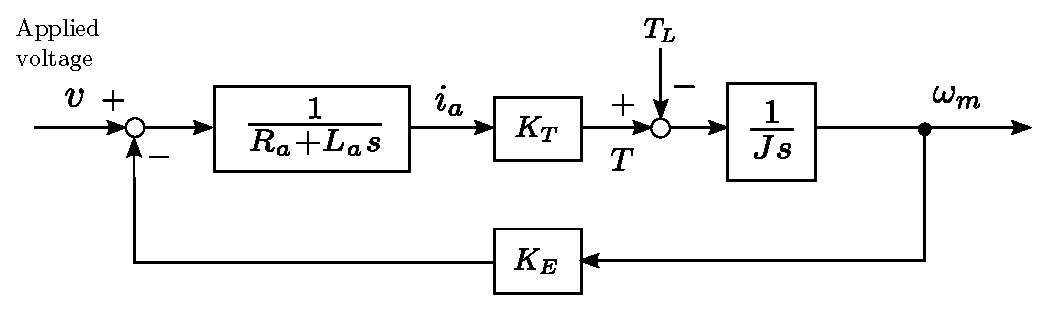
\includegraphics[scale=0.8]{../figure/eps/DCmodel.eps}
  \caption{DCモータのブロック線図}
  \label{DCmodel}
 \end{center}
\end{figure}


\section{LQI速度制御系の設計}
%
目標速度$ \omega _m ^* $を入力するコントローラを用いて,レギュレータと積分器の組み合わせによりサーボ系を構成する.この制御法を LQI (Linear Quadratic Integral)制御と呼ぶ.このブロック線図を{\bf Fig.}\ref{LQI}に示す.
%
\begin{figure}[tb]
 \begin{center}
  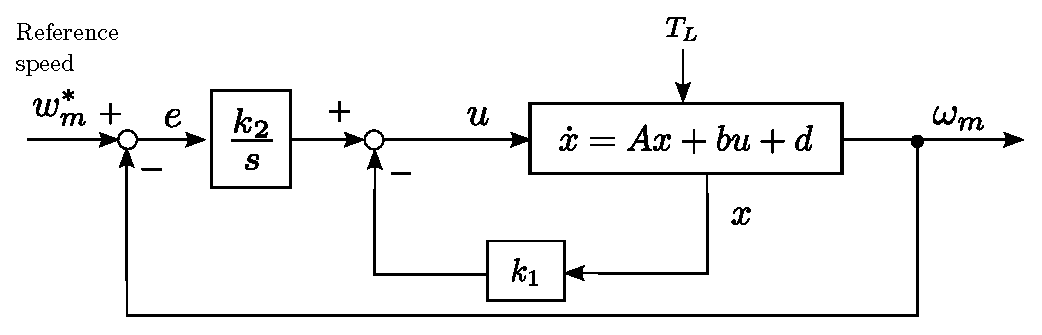
\includegraphics[scale=0.8]{../figure/eps/LQI.eps}
  \caption{LQI 制御系}
  \label{LQI}
 \end{center}
\end{figure}
%
モータの状態方程式は
%
\begin{equation}
 \dfrac{dx}{dt} =
  \left[
   \begin{array}{cc}
    - \dfrac{R_a}{L_a} & - \dfrac{K_E}{L_a} \\
    \dfrac{K_T}{J } & 0 \\
   \end{array}
  \right]
 x +
 \left[
  \begin{array}{c}
   \dfrac{1}{L_a} \\
   0 \\
  \end{array}
 \right]
 u = Ax + bu
\end{equation}
%
ただし,$ x = (i_a \hspace{4mm} \omega_m)^T $で与えられ,係数行列$ A, \hspace{1mm} b $は,
%
\begin{equation}
\begin{array}{c}
 A =
 \left[
  \begin{array}{cc}
   - \dfrac{R_a}{L_a} & - \dfrac{K_E}{L_a} \\
   \dfrac{K_T}{J } & 0 \\
  \end{array}
 \right]
 =
 \left[
  \begin{array}{cc}
   - \dfrac{0.15}{0.003} & -\dfrac{8.50}{0.003} \\
   \dfrac{8.50}{10} & 0 \\
  \end{array}
 \right]
 =
 \left[
  \begin{array}{cc}
   -50 & -2833 \\
   0.85 & 0 \\
  \end{array}
 \right]
\\\\
 b =
 \left[
  \begin{array}{c}
   \dfrac{1}{L_a} \\
   0 \\
  \end{array}
 \right]
 =
 \left[
  \begin{array}{c}
   333 \\
   0 \\
  \end{array}
 \right]
\end{array}
\end{equation}
%
となる.また,出力方程式は
%
\begin{equation}
 y = cx , \hspace{4mm} c = ( 0 \hspace{4mm} 1)
\end{equation}
%
である.そこで,拡大系の状態方程式は,
%
\begin{equation}
 \delta \dot{x}_e = A_e \delta x_e + b_e w
\end{equation}
%
となり,係数行列は,
%
\begin{equation}
 A_e =
 \left[
  \begin{array}{cc}
   A & b \\
   0 & 0 \\
  \end{array}
 \right]
 =
 \left[
  \begin{array}{ccc}
   - 50 & -2833 & 333 \\
   0.85 & 0 & 0 \\
   0 & 0 & 0 \\
  \end{array}
 \right] , \hspace{4mm} b_e =
 \left[
  \begin{array}{c}
   0 \\
   0 \\
   1 \\
  \end{array}
 \right]
\end{equation}
%
と求められ,評価関数は以下のようになる.
%
\begin{equation}
 J_e = \int_0^{\infty} (\delta x_e^T Q_e \delta x_e + r_e w^2) dt
\end{equation}
%
ただし,
%
\begin{equation}
 Q_e = c_e^T c_e = (c \hspace{4mm} 0)^T (c \hspace{4mm} 0) =
 \left[
  \begin{array}{c}
   0 \\
   1 \\
   0 \\
  \end{array}
 \right]
 \left[
  \begin{array}{ccc}
   0 & 1 & 0 \\
  \end{array}
 \right] =
 \left[
  \begin{array}{ccc}
   0 & 0 & 0 \\
   0 & 1 & 0 \\
   0 & 0 & 0 \\
  \end{array}
 \right]
\end{equation}
%

そこで,任意の重み$ r_e $に対して$ LQ $問題を計算する.$ r_e = 0.001 $としたとき,次のリッカチ方程式
%
\begin{equation}
 A_e P_e + P_e A_e + Q_e - P_e b_e b_e^T P_e / r_e
\end{equation}
%
を満たす正定対称解
%
\begin{equation}
 P_e =
 \left[
  \begin{array}{ccc}
   0 & 0.0002 & 0 \\
   0.0002 & 0.0204 & 0.0001 \\
   0 & 0.0001 & 0.0037 \\
  \end{array}
 \right]
\end{equation}
%
を用いて,フィードバックゲイン$ k_e $は
%
\begin{equation}
 k_e = [ 0.0206 \hspace{4mm} 0.1265 \hspace{4mm} 3.7022 ]
\end{equation}
%
と求まる.ここで,
%
\begin{equation}
 Z =
 \left[
  \begin{array}{cc}
   A & b \\
   c & 0 \\
  \end{array}
 \right]
 =
 \left[
  \begin{array}{ccc}
   -50 & -2833 & 333 \\
   0.85 & 0 & 0 \\
   0 & 1 & 0 \\
  \end{array}
 \right]
\end{equation}
%
であるから,重みに対するサーボ系のゲインとして
\begin{equation}
 [k_1 \hspace{4mm} k_2] = k_e Z^{-1} = [0.0111 \hspace{4mm} 0.6782 \hspace{4mm} 31.6230]
\end{equation}
%
を得る.同様に$ r_e = 0.01, ~ 0.1, ~ 1 $のときについて計算すると,次のようになる.
%
\begin{eqnarray}
  \left[ k_1 ~~ k_2 \right] & = & k_e Z^{-1} = [0.0035 ~~ 0.2100 ~~ 10.0001]~~~(r_e = 0.01) \\
  \left[ k_1 ~~ k_2 \right] & = & k_e Z^{-1} = [0.0011 ~~ 0.0659 ~~ 3.1619]~~~~(r_e = 0.1) \\
  \left[ k_1 ~~ k_2 \right] & = & k_e Z^{-1} = [0.0004 ~~ 0.0208 ~~ 0.9996]~~~~(r_e = 1)
\end{eqnarray}


\section{4象限運転シミュレーション}

前節で得たモデルを用いてMATLAB上でシミュレーションを行ない,その結果を出力した.本課題では重みがそれぞれ$ r_e = 0.001, ~ 0.01, ~ 0.1, ~ 1 $のときのシミュレーション結果を{\bf Fig.}\ref{sim1}〜\ref{sim4}に示す.目標速度は運転の開始時より20[s]間隔で変化させ,運転開始時がDCモータの基底速度である500[rpm],そこから0[rpm],-500[rpm],0[rpm]と変動させた.
% $ r_e = 0.001 $に設定した場合は目標速度を捉えられているが,重みが大きくなるにつれて十分な目標速度を得られていないことが分かる.これは,応答速度によるものである.
重みを大きくすると速度,およびトルクの出力応答が遅くなる.これにより,速度の応答も遅くなるため$ r_e = 1 $では十分な目標速度を得られていないことが分かる.

各区間でのトルクと速度の関係を見ていくことにする.0〜20[s]の区間では,正の値のトルクが印加されることで,モータが回転し速度が向上する.したがって前進加速を行なっている.
20〜40[s]の区間では,前進加速を行なっているところに負の値のトルクが印加されることで,速度が低下する.したがってこの区間では前進減速を行なっている.
40〜60[s]の区間では,減速しているモータに対し再び負の値のトルクが印加されることで,速度が負の方向へ変化し,後進加速となる.
60〜80[s]の区間では,ここに正の値のトルクが印加されることにより負の方向の速度が減少し,後進減速となる.
%
\begin{figure}[H]
 \begin{center}
 \hspace{-1.0cm}
  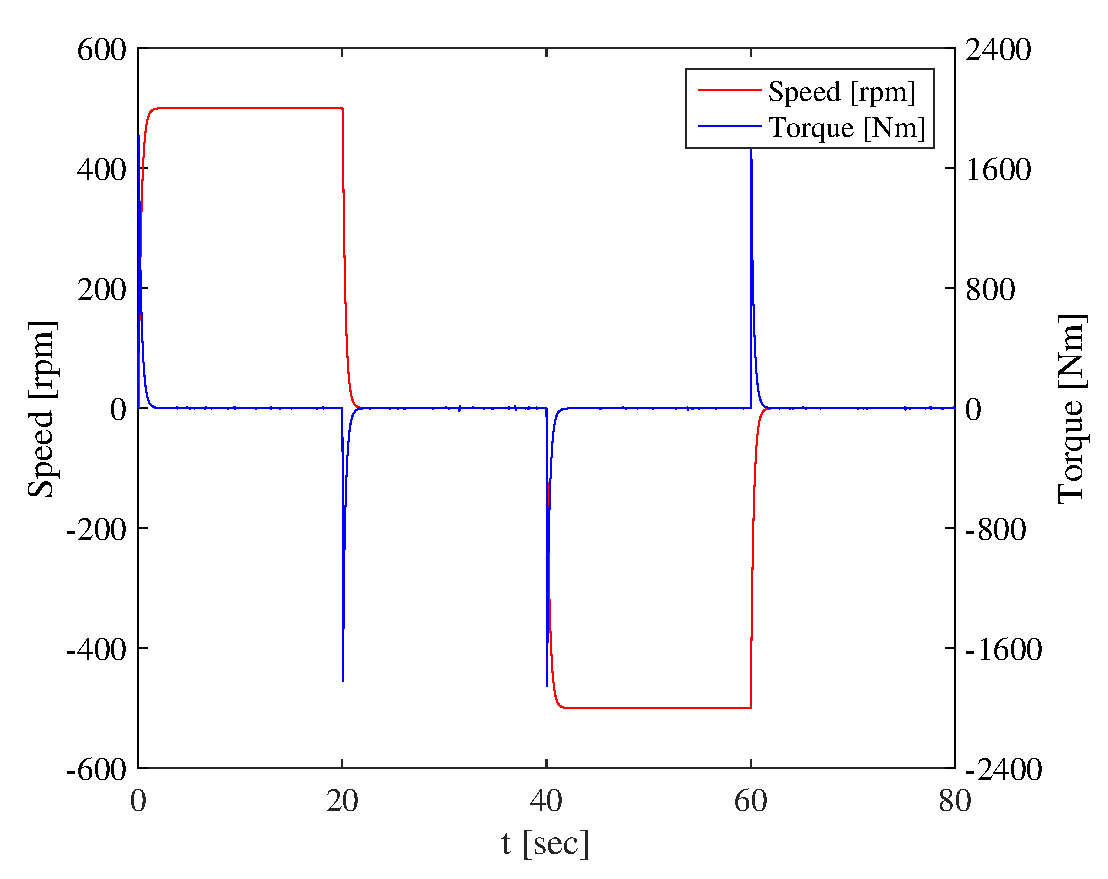
\includegraphics[scale=0.65]{../figure/eps/simout_1.eps}
  \caption{シミュレーション結果($ r_e = 0.001 $)}
  \label{sim1}
 \end{center}

\end{figure}
\begin{figure}[H]
 \begin{center}
 \hspace{-1.2cm}
  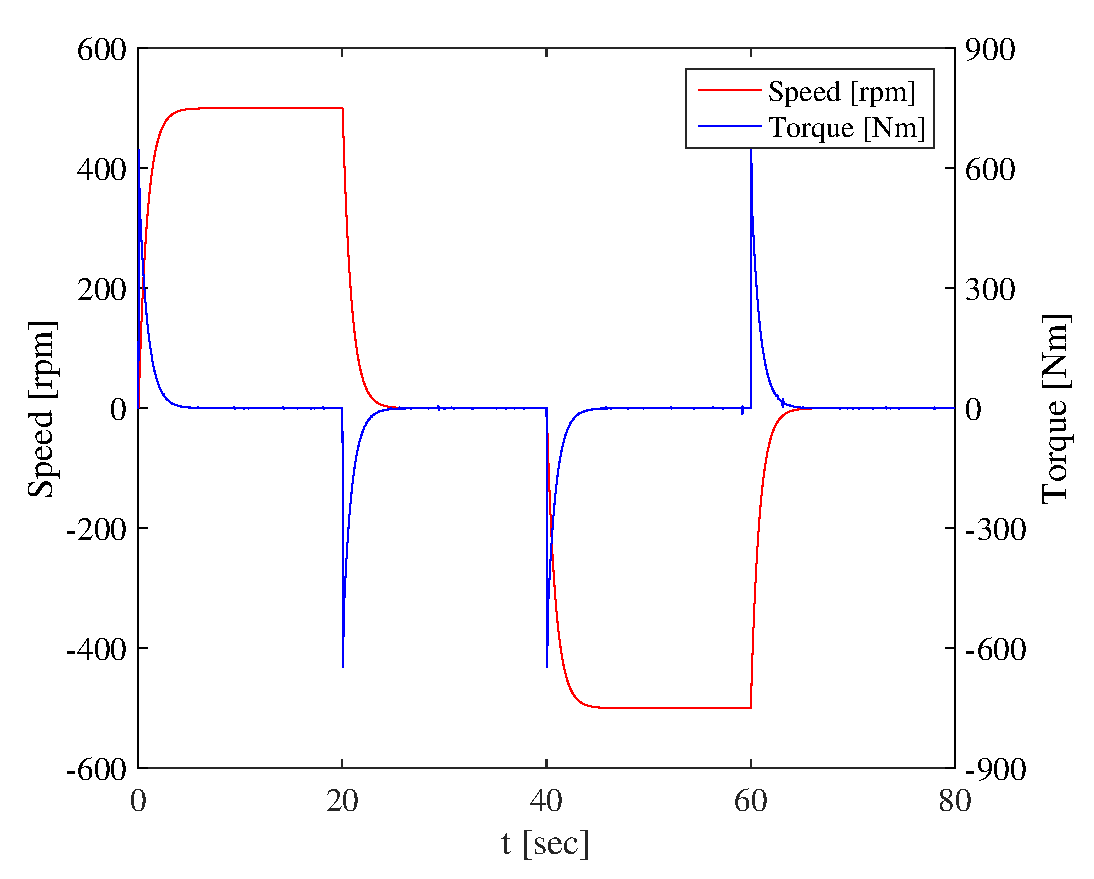
\includegraphics[scale=0.65]{../figure/eps/simout_2.eps}
  \caption{シミュレーション結果($ r_e = 0.01 $)}
  \label{sim2}
 \end{center}
\end{figure}

\begin{figure}[H]
 \begin{center}
 \hspace{-1.2cm}
  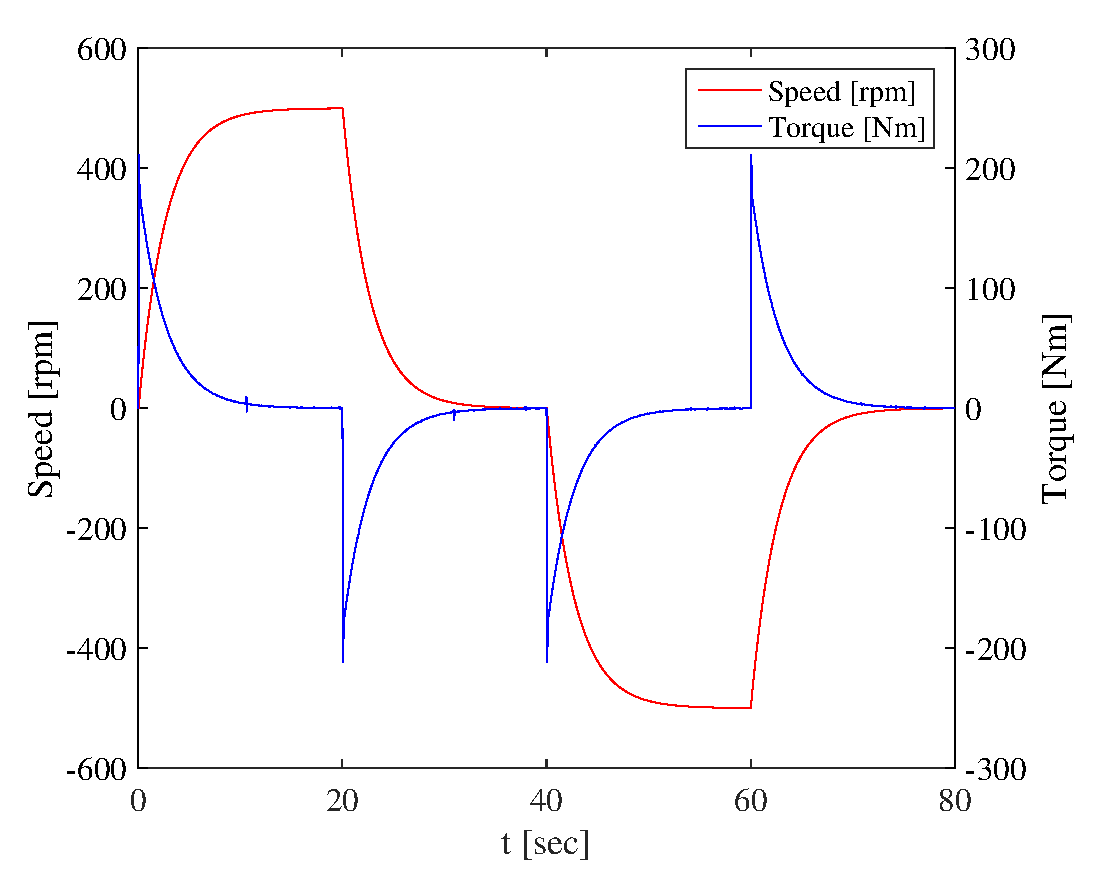
\includegraphics[scale=0.65]{../figure/eps/simout_3.eps}
  \caption{シミュレーション結果($ r_e = 0.1 $)}
  \label{sim3}
 \end{center}
\end{figure}

\begin{figure}[H]
 \begin{center}
 \hspace{-1.5cm}
  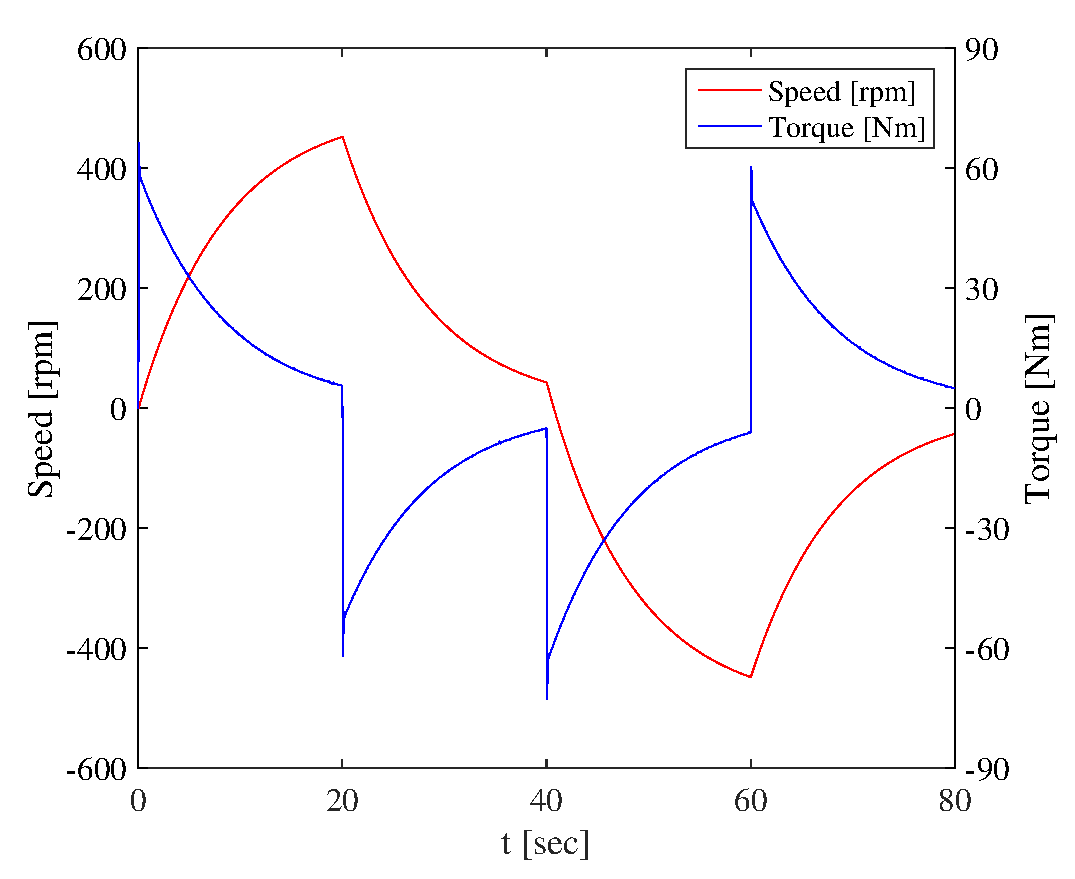
\includegraphics[scale=0.65]{../figure/eps/simout_4.eps}
  \caption{シミュレーション結果($ r_e = 1 $)}
  \label{sim4}
 \end{center}
\end{figure}

\vspace{3cm}
\begin{thebibliography}{99}
\addcontentsline{toc}{section}{参考文献}
\bibitem{1} T.Sakamoto,”Lecture Note of Advanced Electrical Drive Control System”,2017.
\bibitem{2} 坂本 哲三,”電気機器の電気力学と制御”,森北出版,pp.161-191,2007.
% \bibitem{3} 横山 智紀,船渡 寛人,星 新一,吉野 輝雄,”パワーエレクトロニクス学入門”,コロナ社,pp.142-143,2009.
% \bibitem{4} 高木 亮,高見 弘,鳥居 粛,枡川 重男,”基礎から分かる パワーエレクトロニクス講義ノート”,オーム社,pp.118-119,2014.
% \bibitem{5} 佐藤 淳一,”パワー半導体の基本と仕組み”,秀和システム,pp.32-35,2011.
% \bibitem{6} 佐藤 之彦,”パワーエレクトロニクス”,オーム社,pp.15-16,78-80,2012.
\end{thebibliography}

\end{document}
